%!TEX root = ../template.tex
%%%%%%%%%%%%%%%%%%%%%%%%%%%%%%%%%%%%%%%%%%%%%%%%%%%%%%%%%%%%%%%%%%%
%% chapter1.tex
%% NOVA thesis document file
%%
%% Chapter with introduction
%%%%%%%%%%%%%%%%%%%%%%%%%%%%%%%%%%%%%%%%%%%%%%%%%%%%%%%%%%%%%%%%%%%
\typeout{NT FILE chapter5.tex}%

\chapter{Technical Approach}
\label{chap:tech_approach}

This chapter presents the technical approach of the project. It describes the overall architecture, the technologies used, and the reasons for choosing each one. The chapter also explains the modules that make up the system, showing how they work and highlighting their main components. Finally, it discusses the testing strategies used to ensure that each module functions correctly and efficiently.

\section{Architecture}
This section presents the overall architecture, the responsibilities of each layer, and how the APIs and services interact to support the application.

The main objective of this thesis was to develop an online and interactive tool for practicing \gls{ND} exercises. In addition, we considered the possibility of expanding the application to support other types of exercises within the logic domain. After collecting the requirements and keeping future expansion in mind, our first step was to define how the project would be divided and what the main components of the tool would be. Each component was designed to focus on a specific concern while remaining flexible for future functionality. 

To achieve this, we designed a three-tier architecture, which is particularly suitable for online tools where the number of simultaneous users can be highly unpredictable [REF 16 FROM PREP]. By separating concerns into different tiers, the system becomes easier to replicate and maintain. This design also improves reliability by enabling multiple levels of redundancy and simplifies deployment. Furthermore, the layered structure allows the system to handle multiple concurrent users efficiently, as each tier can be scaled or replicated independently.

The following describes the elements of the three-tier architecture and the responsibilities of each:
\begin{itemize}[label={}, leftmargin=0pt]
    \item \textbf{Data (Database):} The data tier stores information in a persistent format. In our tool, this tier is responsible for storing details about the exercises that users can practice. In the future, it will also store additional information about students, including their proficiency levels, progress in exercises, and completed or in-progress proofs and tests. This tier manages data consistency, supports queries from the application tier, and ensures that data can be efficiently retrieved and updated when needed.

    \item \textbf{Application (Server):} The application tier acts as the brain of the system. It handles requests from the presentation tier and generates responses by coordinating with the other tiers. This includes invoking internal APIs via direct function calls and accessing the database for data retrieval or storage. This tier enforces the business logic, controls the workflow of exercises, and mediates between the database and presentation layers, ensuring that the operations requested by users are executed correctly.

    \item \textbf{Presentation (Website):} The presentation tier provides the interface where users interact with the system. At this tier, the graphical interface allows users to practice the \gls{ND} exercises and receive feedback on their progress. This layer manages user interactions, presents feedback in real time, and ensures that all requests to the application tier are correctly processed and displayed.
\end{itemize}

\autoref{fig:architecture} illustrates the flow of our architecture and the modules that compose the application. The architecture is divided into two main groups: on the left, the APIs developed to support the tool, and on the right, the services that implement the three-tier architecture.

The APIs (Application Programming Interfaces) provide standardized interfaces that allow different software components to access functionality or data without requiring knowledge of internal implementation details [REF]. The services, on the other hand, are the specific functions that clients can invoke through the APIs to perform actions or retrieve data [REF].

The first API, the Logic API, provides the core functionalities for logic operations, such as reading and interpreting logical formulas and natural proofs. Its design allows additional logic-related components to be integrated in the future without affecting other parts of the system. The second API, the Feedback API, uses the Logic API to manage the amount of feedback generated. It is kept separate from the Logic API because feedback represents a distinct concern that requires independent handling. This separation of concerns improves code maintainability, extensibility, and clarity. The APIs communicate with each other and with the Server service through direct function calls.

\begin{figure}
    \centering
    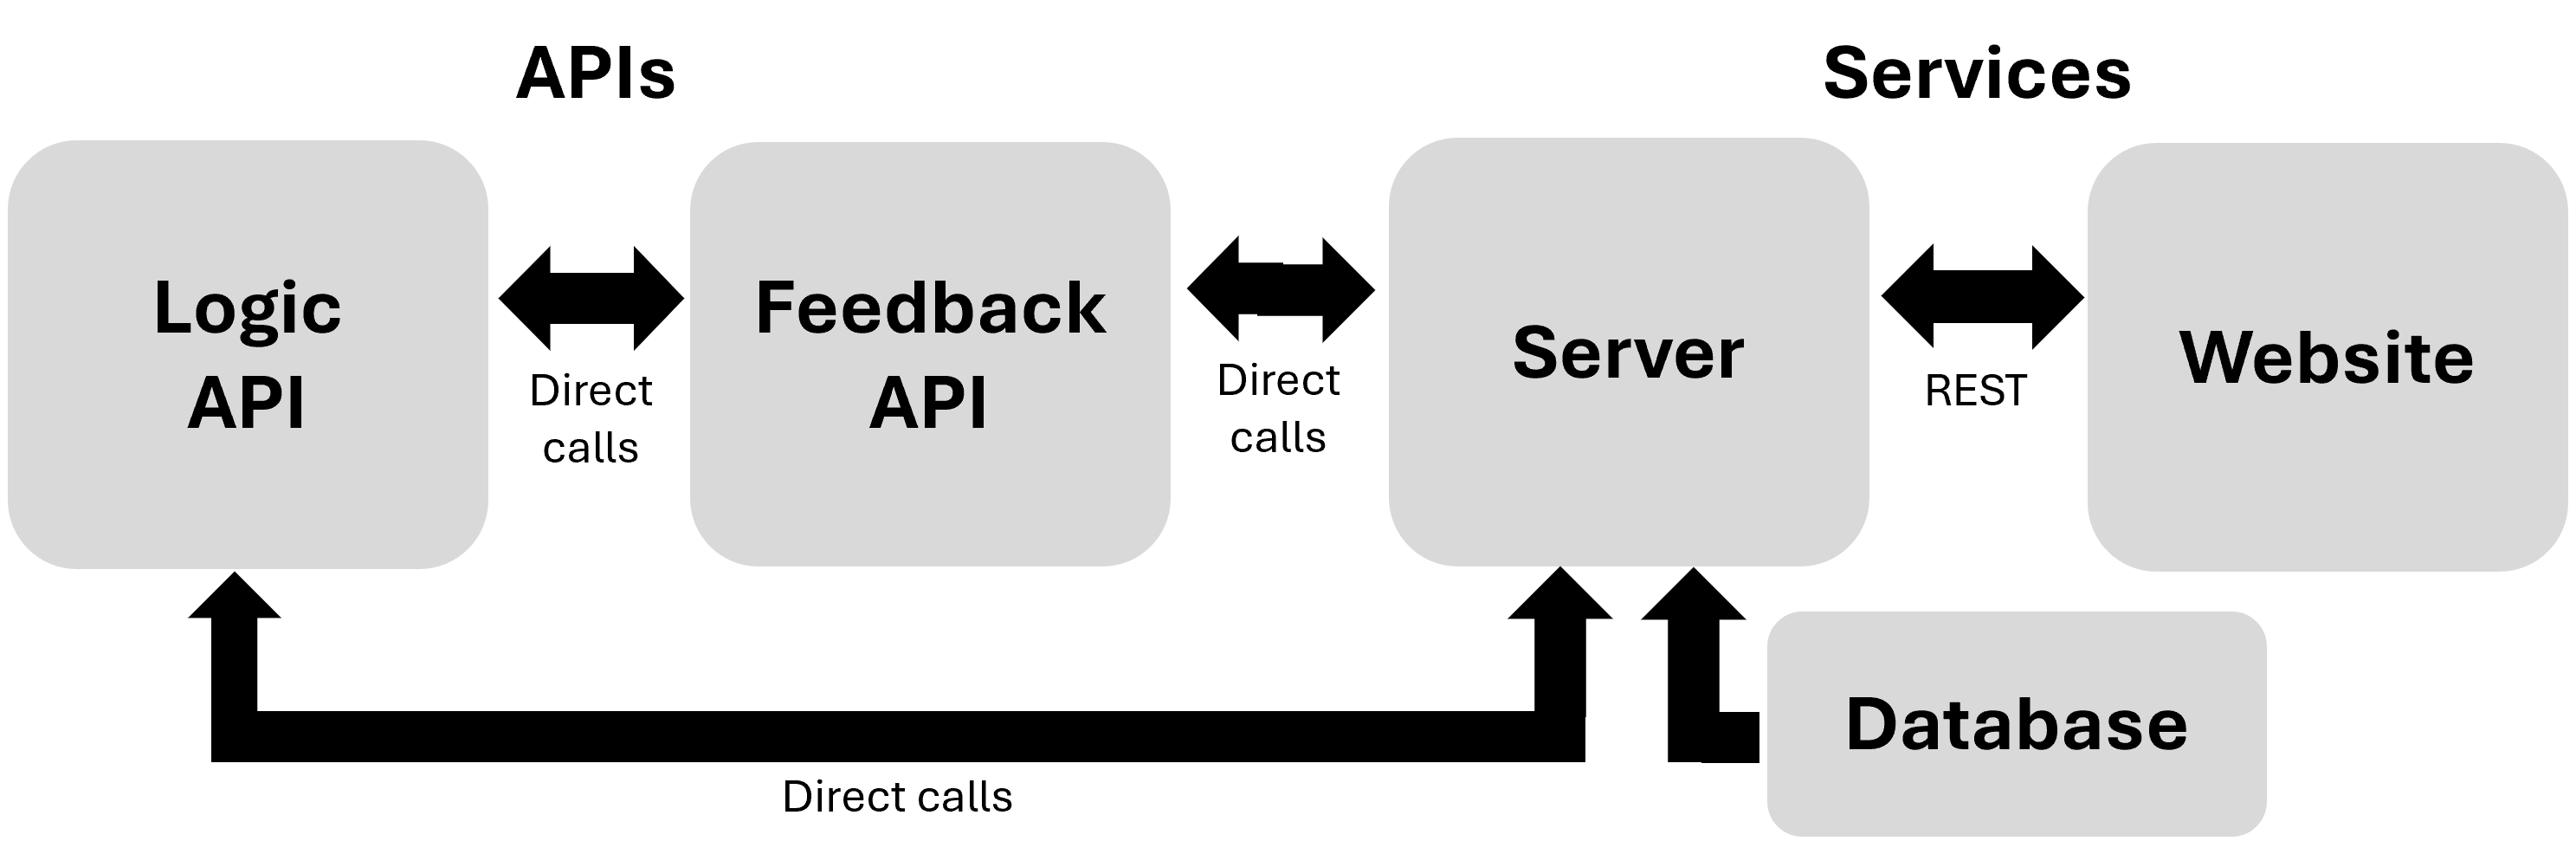
\includegraphics[width=0.95\linewidth]{Chapters/Figures/architeture.png}
    \caption{Architecture of the application, showing the interactions between the different modules.}
    \label{fig:architecture}
\end{figure}

The arrows in \autoref{fig:architecture} represent interactions between the different modules. When a user submits a proof through the Website, the request is sent to the Server. The Server invokes the Feedback API, which calls the Logic API to validate the proof. After receiving the validation result, the Feedback API generates guidance according to the user’s feedback level. The response is then returned to the Server and forwarded to the Website for display.

Another example is when a user requests a list of available exercises. The Website sends the request to the Server, which queries the Data tier to retrieve the exercise information. The Server then formats the data and returns it to the Website, allowing the user interface to dynamically display the available exercises.

A more detailed discussion of these communications is provided in the following sections.

\section{Technologies}
This section presents the technologies and tools used in the development of the application. It highlights the programming languages, frameworks, libraries, and APIs that were selected, along with the rationale behind these choices.

\vspace{1em}
For most modules of the tool, except for the website, we chose Java [REF] as the programming language. We selected Java because it uses an object-oriented approach and we already had experience with it. This helped us develop the tool faster and more easily. Java also makes it easier to reuse and maintain code, which is important for expanding the system in the future.

In the Logic API, in addition to using Java, we employed JavaCC [REF], a parser generator for Java. This tool was very important in the development of our application because it allows user input, such as logical formulas or proofs, to be converted into Java objects. By representing input in this structured way, the system can process it programmatically. JavaCC also performs lexical and syntactic checks, making sure that the input follows the grammar rules of the logic language before any further operations. This reduces errors, improves the reliability of logic operations. Moreover, JavaCC makes it easier to add new grammar rules or logical constructs in the future without affecting other parts of the application.

The Feedback API module is implemented in plain Java, as its main responsibility is to process and manage the errors returned by the Logic API.

Moving to the Server module, we chose the Spring Framework [REF 32]. Spring simplifies web application development by providing a decoupled approach and a range of features that increase productivity [REF 23]. One key advantage is its support for REST APIs, which allows communication with the Website module through HTTP requests and responses and enables data to flow between the different modules of the application. Spring also includes built-in tools for database interactions and transaction management. For the database, we use H2 in memory [REF], as the current data, which consists mainly of exercises, does not require high performance. Spring makes it easy to switch to a more powerful database in the future by changing the configuration. This will allow the system to store more complex information such as user sessions, grading, and other features without interfering with the existing code. Additionally, to generate the endpoints used by the Website layer, we employed Swagger [REF], which automatically creates the necessary API endpoints and integrates them with the server, saving us a significant amount of development time.

In the Website module, the code was written in TypeScript [REF], unlike the other modules. To help us create an interactive tool, we used the React framework [REF 31]. React uses a declarative and component-based approach, which makes the code more intuitive and easier to maintain [REF 18]. Its hierarchical architecture allows developers to build complex pages from smaller, self-contained components, promoting modular and reusable code. Another key feature of React is its ability to efficiently update the user interface in response to state changes, which is especially useful when developing an interactive tool. In addition, we used Redux [REF 9], which provides a centralized data store outside of the React component hierarchy. This reduces system complexity by avoiding the need to pass state through multiple component levels and results in a more organized application structure, making the state easier to manage and maintain. To implement the block-style proof construction, we used the React dnd-kit [REF] and react-zoom-pan-pinch libraries. These libraries provide built-in tools for handling drag-and-drop operations and creating interactive node-based editors, which were essential for implementing the block-style proof construction as we had planned.

Overall, the combination of these technologies allowed us to build a modular, maintainable, and extensible application that supports interactive proof construction efficiently.

\section{Modules}
This section presents the four modules that make up our tool. For each module, we describe its role in the overall application, explain how it functions, highlight its main components, and discuss the testing performed to ensure correctness and reliability.

\subsection{Logic API}
The Logic API module is dedicated entirely to logic and logic operations. It provides the core functionalities for working with formulas in both \gls{PL} and \gls{FOL}, as well as for constructing \gls{ND} proofs in both languages. This was the first module developed, as it provides the foundation for enabling the \gls{ND} exercises. The module is organized into two main parts: one responsible for handling logical formulas, and the other for managing \gls{ND} proofs.

%Dizer aque é um API e que funciona independentemente do resto, o sistema de feedback é limitado aqui referindo-se apenas a pequenos detalhes.
%colocar a interface fornecida nos anexos...

\subsubsection{Formulas}
Formulas in our language are initially provided as character strings. However, their logical structure is hierarchical rather than linear, so a direct textual representation is not sufficient for verification and evaluation purposes. To address this, we use a parser to transform the string into an \gls{AST}. During this process, lexical and syntactic errors are checked before creating the \gls{AST}. The \gls{AST} captures the hierarchical structure of the formula by separating operators and operands into distinct nodes. This provides a structured representation that is independent of the textual notation and can be systematically traversed and analyzed programmatically. The \gls{AST} is essential because it allows us to verify the validity of formulas, extract additional information from them, and provides a foundation for future extensions of the language, such as introducing new logical operators. After creating the \gls{AST}, we construct the final formula object by traversing the tree and extracting relevant information, such as the sets of literals, variables, predicates, and functions. \autoref{fig:flow-exp} shows the steps required to obtain the final formula object.

\begin{figure}[h]
    \centering
    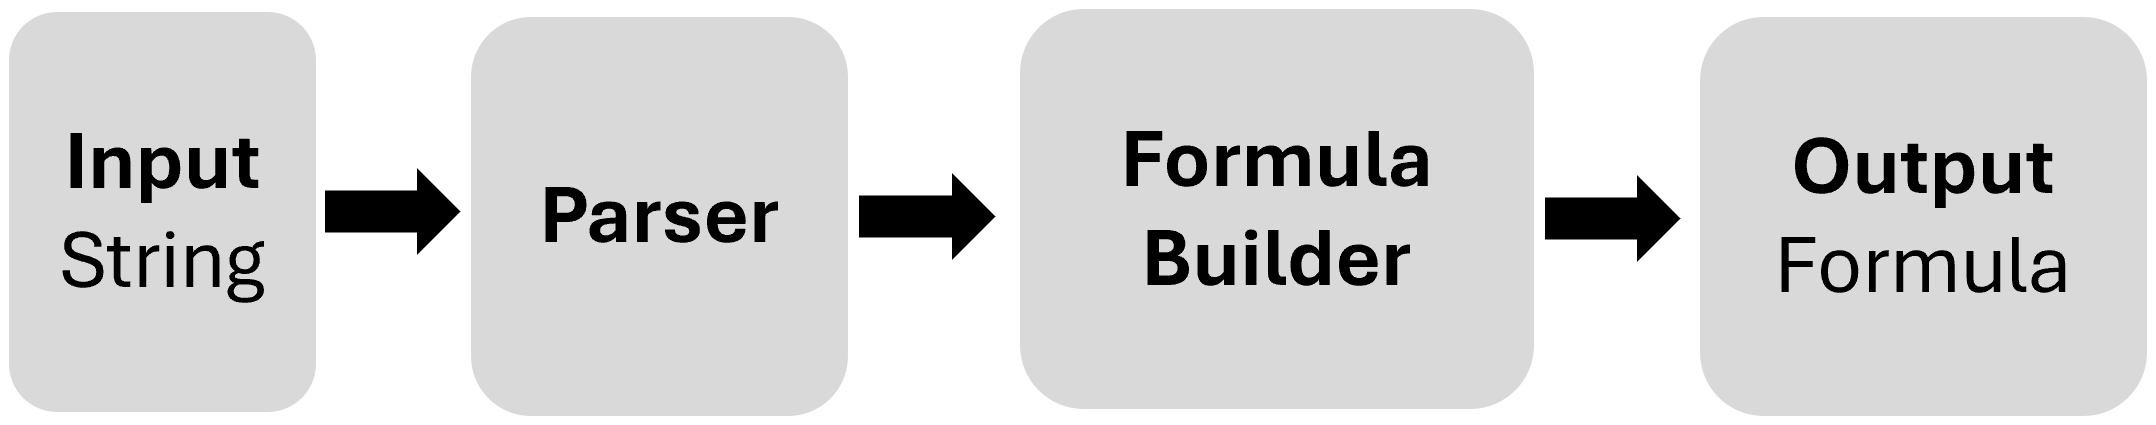
\includegraphics[width=0.85\linewidth]{Chapters/Figures/exp-flow.png}
    \caption{Step-by-step process of creating a formula object from a string input in the system}
    \label{fig:flow-exp}
\end{figure}

Analyzing each step, starting with the parser, as mentioned in the technologies used section, we used JavaCC [REF] to parse the input string into an \gls{AST}. To do this, we first defined the parser rules based on the definitions of \gls{WFF} and the conventions for \gls{PL} and \gls{FOL}. The resulting grammar is presented in \autoref{fig:formulas-syntax}.

\begin{figure}[h!]
\centering
{
\begin{align*}
\text{Predicate } P \quad ::= &\quad [A-Z][a-z,A-Z,0-9]^* \\
\text{Function } f \quad ::= &\quad [a-v] \mid [a-z]([a-z,A-Z,0-9])^+ \\
\text{Variable } x \quad ::= &\quad [w-z] ([0-9])^* \\
\text{Literal } \ell \quad ::= &\quad [a-z] \\
\text{Generic } \alpha \quad ::= &\quad (\phi \mid \delta \mid \psi \mid \alpha \mid \beta \mid \gamma)([0-9])^*\\
\\
\text{Terms } t \quad ::= &\quad x \mid f(t_1, \dots, t_n) \mid f \\
\\
\text{Atomic PL } A_\text{PL} \quad ::= &\quad \top \mid \bot \mid \ell \mid \alpha \\
\text{PL } E_\text{PL} \quad ::= &\quad A_\text{PL} \mid \lnot E_\text{PL} \mid (E_\text{PL} \wedge E_\text{PL}) \\
\mid &\quad (E_\text{PL} \vee E_\text{PL}) \mid (E_\text{PL} \to E_\text{PL}) \mid (E_\text{PL} \leftrightarrow E_\text{PL}) \\
\\
\text{Atomic FOL } A_\text{FOL} \quad ::= &\quad \top \mid \bot \mid x \mid \alpha \mid P(t_1, \dots, t_n) \\
\text{FOL } E_\text{FOL} \quad ::= &\quad A_\text{FOL} \mid  \lnot E_\text{FOL} \mid (E_\text{FOL} \wedge E_\text{FOL}) \\
\mid &\quad (E_\text{FOL} \vee E_\text{FOL}) \mid (E_\text{FOL} \to E_\text{FOL}) \mid (E_\text{FOL} \leftrightarrow E_\text{FOL}) \\
\mid &\quad \forall x. E_\text{FOL} \mid \exists x. E_\text{FOL}
\end{align*}
}
\caption{Grammar for the syntax for Propositional and First-Order Logic.}
\label{fig:formulas-syntax}
\end{figure}

For the \gls{AST}, we defined a hierarchy of classes, as shown in \autoref{fig:exp-asts}. We organized the operations into three types: atomic expressions, unary operations, and binary operations. For each type, we created the corresponding subclasses.

\begin{figure}
    \centering
    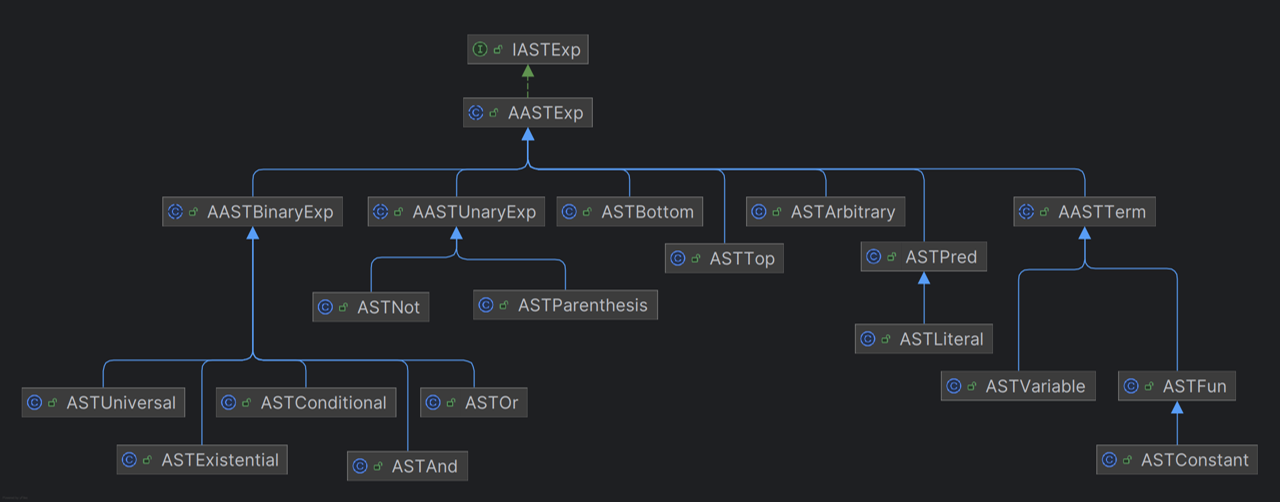
\includegraphics[width=0.95\linewidth]{Chapters/Figures/ast-exp.png}
    \caption{Class diagram showing the Abstract Syntax Tree nodes and their relationships for formulas}
    \label{fig:exp-asts}
\end{figure}

Finally, after creating the formula object by iterating over the \gls{AST} and extracting relevant information, we can perform several operations on the formulas. These operations can be grouped into three main categories:

\begin{itemize}
    \setlength{\itemsep}{5pt}
    \item \textbf{General Operations:} 
    \begin{itemize}[noitemsep, topsep=0pt]
        \item Obtain the full \gls{AST}.
        \item Iterate over generic symbols (Greek letters used as placeholders for abstraction).
        \item Replace symbols in the formula with other formulas (useful for substituting generics and mapping variables).
    \end{itemize}

    \item \textbf{Operations for \gls{PL}:}
    \begin{itemize}[noitemsep, topsep=0pt]
        \item List all unique literals in the formula.
        \item Assign an interpretation and compute the resulting truth value.
        \item Generate the full truth table.
        \item Check equivalence between two formulas based on their truth tables.
    \end{itemize}

    \item \textbf{Operations for \gls{FOL}:}
    \begin{itemize}[noitemsep, topsep=0pt]
        \item Iterate over terms, predicates, formulas, and variables.
        \item Iterate over bounded and unbounded variables (important for checking \gls{ND} proof side conditions).
        \item Check whether a variable is free.
    \end{itemize}
\end{itemize}

There are many other operations that could be included within the scope of logic. However, since the project we developed is focused specifically on \gls{ND} exercises, we only implemented the operations necessary to work with them. Nevertheless, the system is designed in a way that allows easy expansion to support additional operations on formulas, making it possible to extend the system to other types of exercises in the future.

\subsubsection{Natural Deduction Proofs}
For \gls{ND} proofs, we follow a similar approach as with formulas, but with an important difference. While formulas already have a standard linear representation, the proofs we consider are tree-shaped structures and do not have a straightforward linear form. Therefore, we needed to define a specific language to represent \gls{ND} proofs.

We had to define a way to represent proofs in a linear format. This step was crucial because it allows us to detect all possible errors in proofs, while syntactic errors can be handled more easily at the parser level. Although our final online tool checks only for semantic errors, as the layout of rules is already provided, we designed the system to be flexible. This flexibility will allow less restricted proof representations in the future. For example, users could provide the full construction of a proof by specifying the structure of the rules applied, including the number of hypotheses and the number of marks each rule can have.

After passing through the parser, the system checks whether the proof is valid. This process is divided into several substeps, each responsible for verifying a different aspect of the proof and ensuring its semantic correctness. During this phase, the \gls{AST} nodes are enriched with additional relevant information required for the next steps. Finally, using the enriched \gls{AST}, we build the proof object. \autoref{fig:flow-nd} shows the steps required to obtain the final proof object.

\begin{figure}[h]
    \centering
    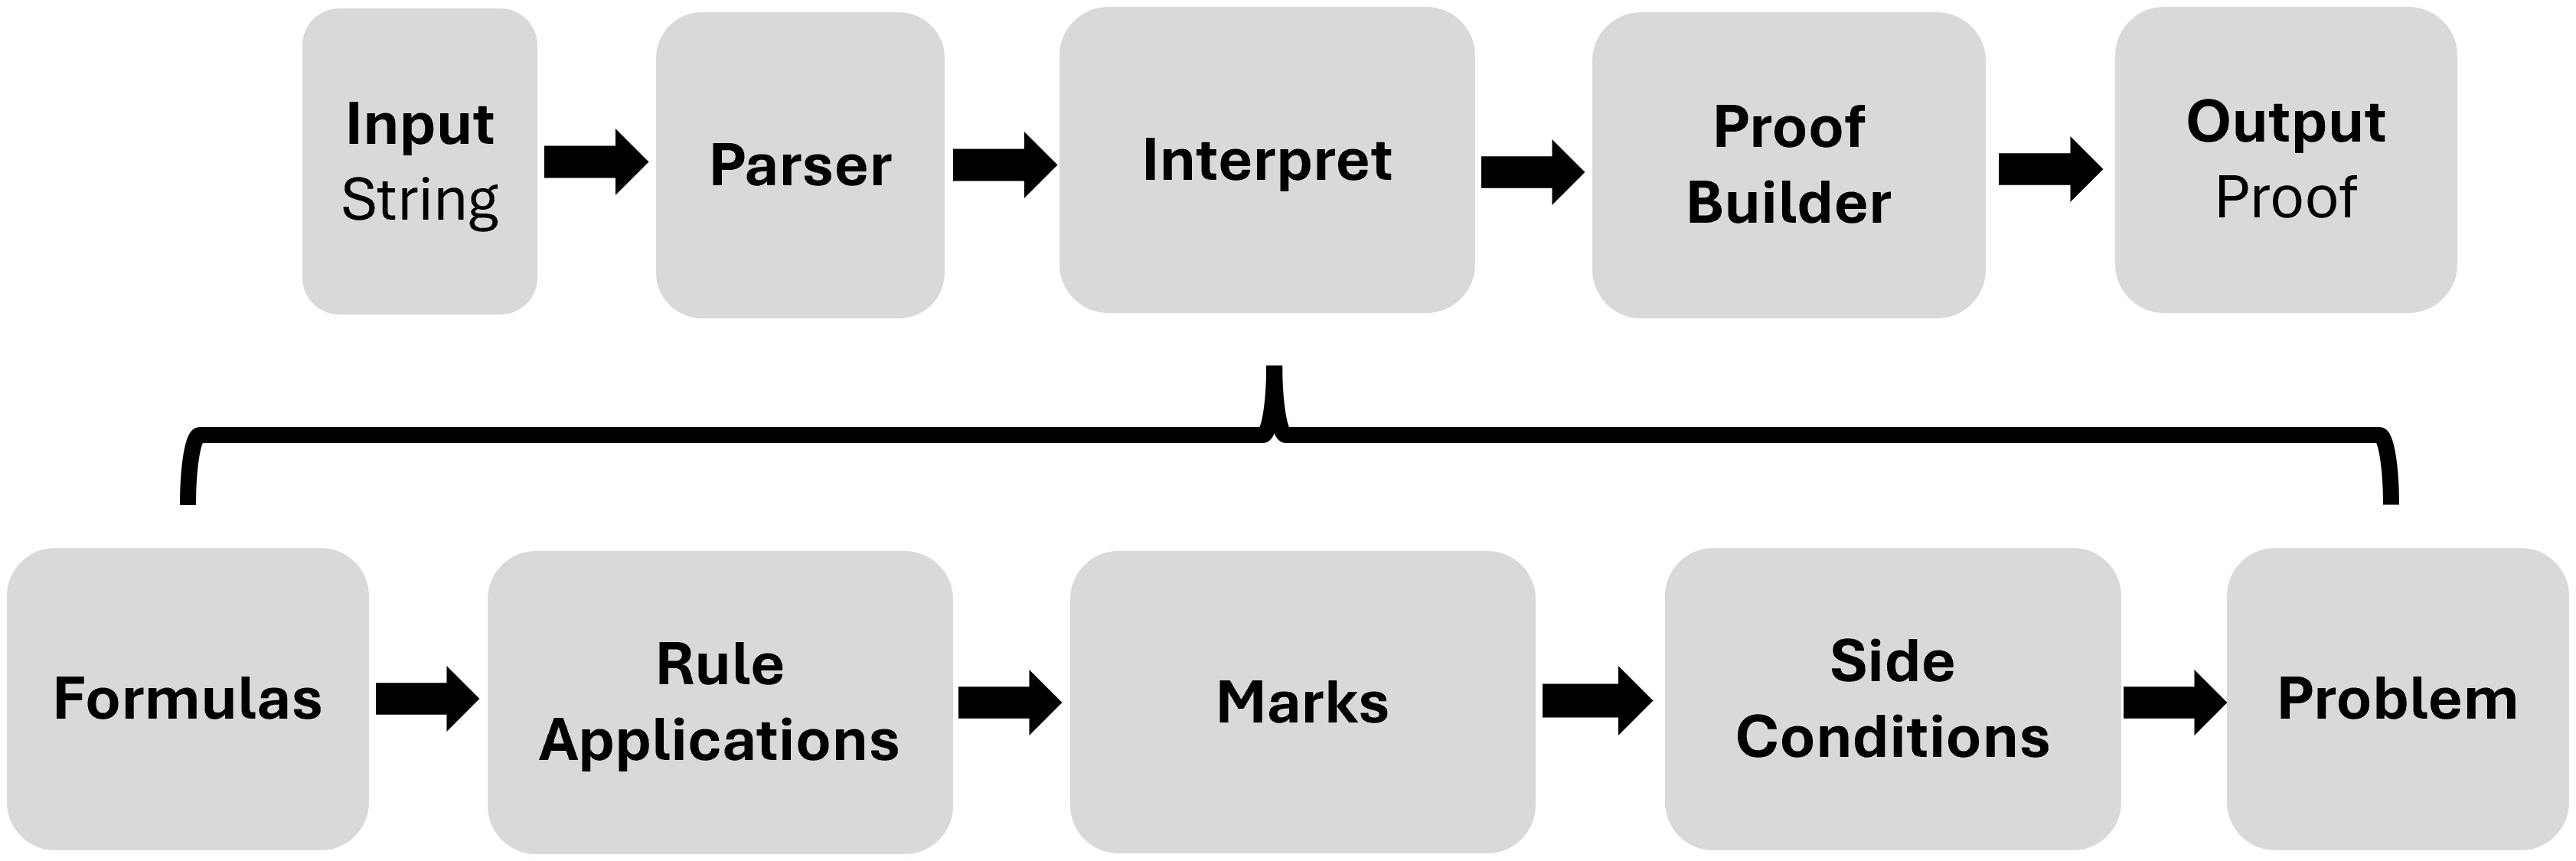
\includegraphics[width=0.95\linewidth]{Chapters/Figures/nd-flow2.png}
    \caption{Step-by-step process of creating a proof object from a string input in the system, including the sub-steps performed by the interpreter}
    \label{fig:flow-nd}
\end{figure}

Analyzing each step, starting with the parser. For that we had to find a way to represent the proofs in a linear way and we ended up with the following representation for the rule application:
\[
    [rule, marks...] [conclusion.\; hypotheses...]
\]
On the left, we have the rule name followed by marks, which appear when the rule closes marks. Next comes the conclusion of the rule, followed by the hypotheses that the rule requires. Let us present the grammar for our representation to keep things a little more clear, see \autoref{parser:nd}. We use the previously presented grammar for formulas within this grammar to indicate how formulas are placed within the rules.

\begin{figure}[H]
\centering
{
\begin{align*}
\text{Number } m \quad ::= &\quad [0-9]^* \\
R_\text{PL} \quad ::= &\quad [\bot, m]\ [E_\text{PL}.\;R_\text{PL}] \\
       \mid &\quad [\lnot I, m]\ [E_\text{PL}.\;R_\text{PL}] \mid [\lnot E]\ [\bot.\;R_\text{PL}\ R_\text{PL}] \\
       \mid &\quad [\land El]\ [E_\text{PL}.\;R_\text{PL}] \mid [\land Er]\ [E_\text{PL}.\;R_\text{PL}] \mid [\land I]\ [E_\text{PL}.\;R_\text{PL}\ R_\text{PL}] \\
       \mid &\quad [\lor Il]\ [E_\text{PL}.\;R_\text{PL}] \mid [\lor Ir]\ [E_\text{PL}.\;R_\text{PL}] \\
       \mid &\quad [\lor E, m, m]\ [E_\text{PL}.\;R_\text{PL}\ R_\text{PL}\ R_\text{PL}] \\
       \mid &\quad [\to\!I, m]\ [E_\text{PL}.\;R_\text{PL}] \mid [\to\!E]\ [E_\text{PL}.\;R_\text{PL}\ R_\text{PL}] \\
       \mid &\quad [H, m]\ [E_\text{PL}.] \\
\\
R_\text{FOL} \quad ::= &\quad [\bot, m]\ [E_\text{FOL}. R_\text{FOL}] \\
       \mid &\quad [\lnot I, m]\ [E_\text{FOL}.\;R_\text{FOL}] \mid [\lnot E]\ [\bot.\;R_\text{FOL}\ R_\text{FOL}] \\
       \mid &\quad [\land El]\ [E_\text{FOL}.\;R_\text{FOL}] \mid [\land Er]\ [E_\text{FOL}.\;R_\text{FOL}] \\
       \mid &\quad [\land I]\ [E_\text{FOL}.\;R_\text{FOL}\ R_\text{FOL}] \\
       \mid &\quad [\lor Il]\ [E_\text{FOL}.\;R_\text{FOL}] \mid [\lor Ir]\ [E_\text{FOL}.\;R_\text{FOL}] \\
       \mid &\quad [\lor E, m, m]\ [E_\text{FOL}.\;R_\text{FOL}\ R_\text{FOL}\ R_\text{FOL}] \\
       \mid &\quad [\to\!I, m]\ [E_\text{FOL}.\;R_\text{FOL}] \mid [\to\!E]\ [E_\text{FOL}.\;R_\text{FOL}\ R_\text{FOL}] \\
       \mid &\quad [\forall I]\ [E_\text{FOL}.\;R_\text{FOL}] \mid  [\forall E]\ [E_\text{FOL}F.\;R_\text{FOL}] \\
       \mid &\quad [\exists I]\ [E_\text{FOL}.\;R_\text{FOL}] \mid [\exists E, m]\ [E_\text{FOL}.\;R_\text{FOL}\ R_\text{FOL}] \\
       \mid &\quad [H, m]\ [E_\text{FOL}.]
\end{align*}
}
\caption{Grammar for the syntax for Natural Deduction Proofs}
\label{parser:nd}
\end{figure}

For every logic symbol, depending on the logic language we are using, there is a way to express the corresponding set of rules. In addition to the rules for each logic symbol, there is a special rule, represented as \(H\), that is used to assign marks to formulas. We chose this design to represent proofs because it is similar to the rules presented in [REF RULES]. By using tab indentation, we can create a structure that resembles these rules. The main difference lies in the orientation of the proof: in our representation, the proof always starts from the conclusion and grows downward as more rules are applied.

Although the language was defined specifically for \gls{ND} in \gls{PL} and \gls{FOL}, the modular structure of the grammar makes it possible to extend it with additional rules or logical operators without changing the overall design.

Let us show some examples of proofs represented in both ways, using our language and the standard tree-shaped representation. In our first example, we want to prove \(\{(p \to q) \to p\} \vdash q \to p\). In the representation shown in \autoref{parser:nd_firs_ex}, the left side displays the full proof using our language. The proof starts from the conclusion and as the rules are applied, indentation is used to structure it. The indentation is not part of the language but helps make the proof easier to read instead of writing everything in a single line. On the right side of the image, the same proof is shown using the traditional tree-shaped representation.

\begin{figure}[H]
\centering
{\scriptsize
\begin{minipage}[t]{0.48\textwidth}
\centering
\begin{lstlisting}[basicstyle=\ttfamily\scriptsize, escapeinside={(*@}{@*)}]
[(*@$\to$@*)I,2] [q (*@$\to$@*) p.
  [(*@$\to$@*)E] [p.
    [(*@$\to$@*)I,3] [p (*@$\to$@*) q.
      [H,2] [q.]]
    [H,1] [(p (*@$\to$@*) q) (*@$\to$@*) p.]]]
\end{lstlisting}
\end{minipage}
\hfill
\begin{minipage}[t]{0.48\textwidth}
\centering
\begin{prooftree}
  \AxiomC{${q}^2$}
  \RightLabel{$(\to_I)$}
  \UnaryInfC{$p \to q$}
  
  \AxiomC{${(p \to q) \to p}^1$}
  
  \RightLabel{$(\to_E)$}
  \BinaryInfC{$p$}
  \RightLabel{$(\to_I,2)$}
  \UnaryInfC{$q \to p$}
\end{prooftree}
\end{minipage}
}
\caption{Example of a proof in Propositional Logic using our own Natural Deduction language}
\label{parser:nd_firs_ex}
\end{figure}

In the second example, we show a proof in \gls{FOL}, displayed in \autoref{parser:nd_sec_ex}. In this case, we want to prove \(\{\exists y \; \forall x \;\phi\} \vdash \forall x \;\exists y \;\phi\).

\begin{figure}[H]
\centering
{\scriptsize
\begin{minipage}[t]{0.48\textwidth}
\centering
\begin{lstlisting}[basicstyle=\ttfamily\scriptsize, escapeinside={(*@}{@*)}]
[(*@$\exists$@*)E,2] [(*@$\forall x$@*) (*@$\exists y$@*) (*@$\phi$@*).
    [H,1] [(*@$\exists y$@*) (*@$\forall x$@*) (*@$\phi$@*).]
    [(*@$\forall$@*)I] [(*@$\forall x$@*) (*@$\exists y$@*) (*@$\phi$@*).
        [(*@$\exists$@*)I] [(*@$\exists y$@*) (*@$\phi$@*).
            [(*@$\forall$@*)E] [(*@$\phi$@*).
                [H,2] [(*@$\forall x$@*) (*@$\phi$@*).]]]]]
\end{lstlisting}
\end{minipage}
\hfill
\begin{minipage}[t]{0.48\textwidth}
\centering
\begin{prooftree}
  \AxiomC{${\exists y \; \forall x \;\phi}^1$}

  \AxiomC{${\forall x \;\phi}^2$}
  \RightLabel{$(\forall_E)$}
  \UnaryInfC{$\phi$}
  \RightLabel{$(\exists_I)$}
  \UnaryInfC{$\exists y \;\phi$}
  \RightLabel{$(\forall_I)$}
  \UnaryInfC{$\forall x \;\exists y \;\phi$}
  \RightLabel{$(\exists_E,2)$}
  \BinaryInfC{$\forall x \;\exists y \;\phi$}
\end{prooftree}
\end{minipage}
}
\caption{Example of a proof in First-Order Logic using our own Natural Deduction language}
\label{parser:nd_sec_ex}
\end{figure}

For the AST, similarly to formulas, we defined a hierarchy of classes, as shown in \autoref{fig:nd-asts}. The classes are organized into three types: unary rules, binary rules, and a category for the disjunction rule and the hypothesis. For each type, we created the corresponding subclasses. By structuring the classes in this way, we can inherit fields from parent classes, avoiding code duplication.

\begin{figure}
    \centering
    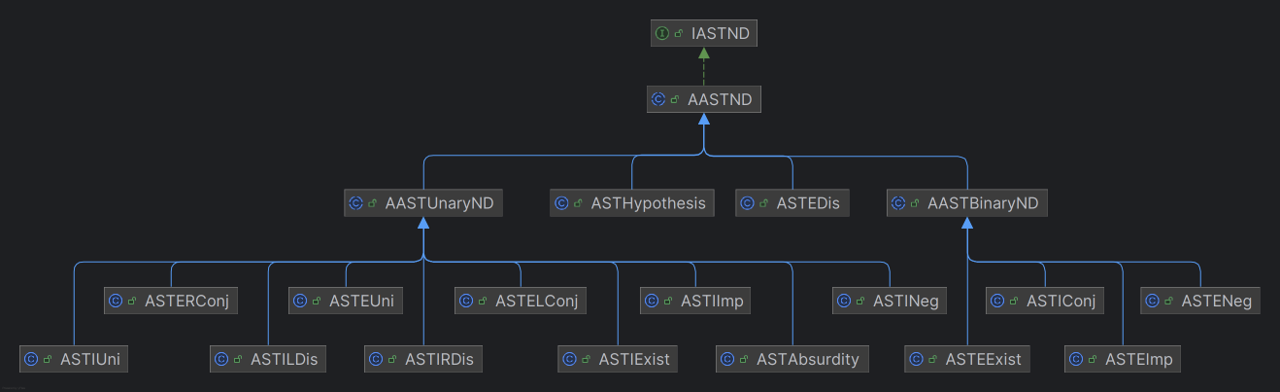
\includegraphics[width=0.95\linewidth]{Chapters/Figures/ast-nd.png}
    \caption{Class diagram of the Abstract Syntax Tree nodes for proofs.}
    \label{fig:nd-asts}
\end{figure}

Focusing now on the interpreter, it is divided into five sequential steps, each responsible for a different task to ensure that the proof is semantically correct. We describe each step below:

\begin{itemize}[noitemsep, topsep=0pt]
    \setlength{\itemsep}{5pt}
    \item \textbf{Formulas:} In the first step, the interpreter converts the formulas that make up the proof into actual formula objects. This involves iterating over all formulas and executing the procedure presented in \autoref{fig:flow-exp}. This step is crucial for the subsequent processes, as we need to extract information from the formulas to ensure that the proof is correct.

    \item \textbf{Rule Applications:} This step ensures that each rule application is correct. It verifies that the applied rules follow the structure defined in [REF RULES], guaranteeing that the conclusion can be logically derived from the corresponding set of hypotheses. Additionally, it keeps track of the assumptions made in each rule and stores this information in the corresponding rule node of the \gls{AST}.
    
    \item \textbf{Marks:} Here, we check for conflicts in marks. Specifically, we ensure that no formula has multiple marks, that no mark references multiple formulas, and that the marks can indeed be used to close the applied rules. We also track which hypotheses are open and which are closed.
    
    \item \textbf{Side Conditions:} In this step, we verify that all rules satisfy their respective side conditions.
    
    \item \textbf{Problem:} This final step is optional and applies only when interpreting a proof under a specific problem. It checks whether the proof solves the problem by checking that the conclusion of the proof matches the conclusion of the problem and that the set of premises in the proof is contained within the set of premises of the problem.
\end{itemize}

Finally, after ensuring that the proof is semantically correct, we can create the proof object by iterating over the \gls{AST} and extracting relevant information about the proof. From the proof object, we can perform several operations on the formulas. Some of these operations are listed below:

\begin{itemize}[noitemsep, topsep=0pt]
    \item \textbf{General Operations:}
    \begin{itemize}[noitemsep, topsep=0pt]
        \item Obtain the full \gls{AST} of the proof.
        \item Retrieve the conclusion.
        \item Iterate over the hypotheses and its marks.
        \item Iterate over the premises.
        \item Get the total number of rules applied.
        %\item Get the number of leaves.
    \end{itemize}
\end{itemize}

This module provides a basic interface focused specifically on \gls{ND} proofs, rather than the full scope of logic operations. Nevertheless, it is built on a solid foundation that can be easily extended to support additional operations in the future. By implementing this module as a separate component within the overall application, the system achieves a clear separation of concerns, making it easier to maintain and test. Moreover, this modular design facilitates future expansion: new operations, rules can be added without affecting other parts of the application. The separation also allows other modules or tools to reuse the logic independently, supporting the development of additional features or extensions in the domain of logical reasoning and formal proofs.

\subsubsection{Tests}

The logic module was tested using JUnit [REF] tests. For formulas, we created a representative set covering various types of errors, including missing parentheses, ambiguities, invalid tokens, and missing symbols. For proofs, we used our own test grammar representation, to test some of the exercises presented in [REF ANNEX]. For certain exercises, we provided the correct solutions, while for others we simulated the most common errors made by students. Examples include violations of side conditions, conflicts between marks, and failure to close marks properly.


\subsection{Feedback API}
This module is responsible for handling feedback messages. On the Logic API module, logic errors are thrown but never properly processed, they typically result in generic error messages that do not provide detailed information about what happened. The purpose of the Feedback module is to enrich these messages and attach them to formulas and proofs, based on the user's feedback level.  

Initially, this module did not exist, and exceptions were handled directly within the Logic API. However, we realized that feedback and feedback levels are concepts outside the logic domain. By moving them to a dedicated module, we achieve a clear separation of concerns, which improves code maintainability and readability. This separation also makes it easier to extend or modify the feedback system in the future without affecting the core logic of the proofs.

\subsubsection{Process}
In this module, we first compute the formula or the proof object using the previous API. We then convert the returned objects into a different representation, allowing feedback messages and other relevant information to be assigned to the various elements that make up a proof.

Errors can be assigned to formulas, where the question mark appears next to the formula, or to rules, where the question mark appears on the left side of the rule application. The current feedback API supports not only messages but also previews of proof trees, allowing for richer feedback. In the feedback shown in \autoref{fig:nd-asts}, a message is sent along with a preview of a possible mark that can be used.

\begin{figure}
    \centering
    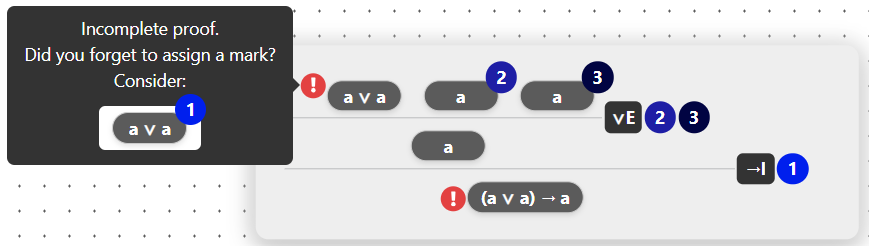
\includegraphics[width=0.75\linewidth]{Chapters/Figures/feed-error.png}
    \caption{Example of a proof with feedback messages and previews.}
    \label{fig:nd-asts}
\end{figure}

\autoref{lst:feed-json} shows the JSON produced after checking the proof, with some fields omitted for simplicity. Note that this JSON representation is not the final form sent to the website, that process will be covered in detail in the next module. In this representation, multiple feedback messages can be assigned to each part of the object, allowing the proof to display more than one message at once. Previews, which are also proof objects, can be attached to the feedback.

Additionally, the object can store other relevant information to facilitate feedback in the application. For example, for each formula, we track the visible assumptions at that point in the proof. In the case of the formula displaying an error in the figure, the environment, which is the set of assumptions available at that stage, is \(a \land a\) and is assigned to mark 1. This is extremely useful for helping users recall which assumptions have been made. In the interface, we can display at any moment which marks and their corresponding formulas are available for use.

\begin{figure}[H]
\centering
\begin{minipage}{0.48\textwidth}
\begin{lstlisting}[language=json,
numbers=left]
{
  "conclusion": {
    "feedback": "This tree doesn't solve the problem!\nYou proved:\n{a ∨ a} ⊢ (a ∨ a) → a",
    "exp": "(a ∨ a) → a",
    "previews": [],
    "marks": ["1"],
    "rule": "INTRO_IMPLICATION",
    "hypotheses": [
      {
        "conclusion": { "exp": "a" },
        "marks": ["2", "3"],
        "rule": "ELIM_DISJUNCTION",
        "hypotheses": [
          {
            "feedback": "Incomplete proof.\nDid you forget to assign a mark?\nConsider:",
\end{lstlisting}
\end{minipage}%
\hfill
\begin{minipage}{0.48\textwidth}
\begin{lstlisting}[language=json,
numbers=left,
firstnumber=last]
            "previews": [
              {
                "conclusion": {
                  "exp": "a ∨ a"
                },
                "marks": ["1"],
                "rule": "HYPOTHESIS",
                ...
              }
            ],
            "env": { "1": "a ∨ a" }
          },
          ...
        ]
      }
    ]
  }
}
\end{lstlisting}
\end{minipage}
\caption{Example of the feedback JSON representation of a proof}
\label{lst:feed-json}
\end{figure}

Moreover, this module is where our algorithm for generating automatic proofs was implemented. A detailed explanation and implementation of the algorithm can be found in [REF ALGO]. Using the algorithm, we can extract complete solutions for problems and use these solutions to provide feedback to end users by attaching messages to the relevant parts of the proof where guidance is needed.

The feedback messages in our system were created to guide users while keeping the focus on learning. To design them, we studied other online tools that provide feedback on proofs and exercises. We looked at how they give hints, show errors, or suggest solutions, and we adapted some of these ideas to fit our system. We considered different feedback levels, so that users receive help according to their needs. At lower levels, messages give small hints or point out mistakes without giving the solution. At higher levels, messages can give more guidance or suggest possible answers, but always with the goal of supporting learning rather than just providing solutions. This process helped us create messages that are clear, helpful, and suitable for different levels of feedback, allowing users to learn step by step while interacting with the proof.

\subsubsection{Tests}
This module of our system was primarily evaluated through user testing sessions [REF USER-TESTING] to understand whether the reported errors were clear, helpful, and guided users toward correct reasoning. The algorithm was tested for correctness by comparing its output with reference exercises and verified through unit tests of both the ND proof interpreter and the algorithm itself. Additionally, performance was monitored to track memory usage and execution time, allowing us to identify and address potential bottlenecks [REF ALGO TESTS].

\subsection{Server and Database Services}
The Server module is responsible for communicating with the database and the website via REST requests, generating responses by coordinating with the other modules. This includes invoking internal APIs through direct function calls and accessing the database for data retrieval. The internal structure of this layer is divided into three layers. \autoref{fig:server-modules} illustrates these layers and how they are organized.

\begin{figure}
    \centering
    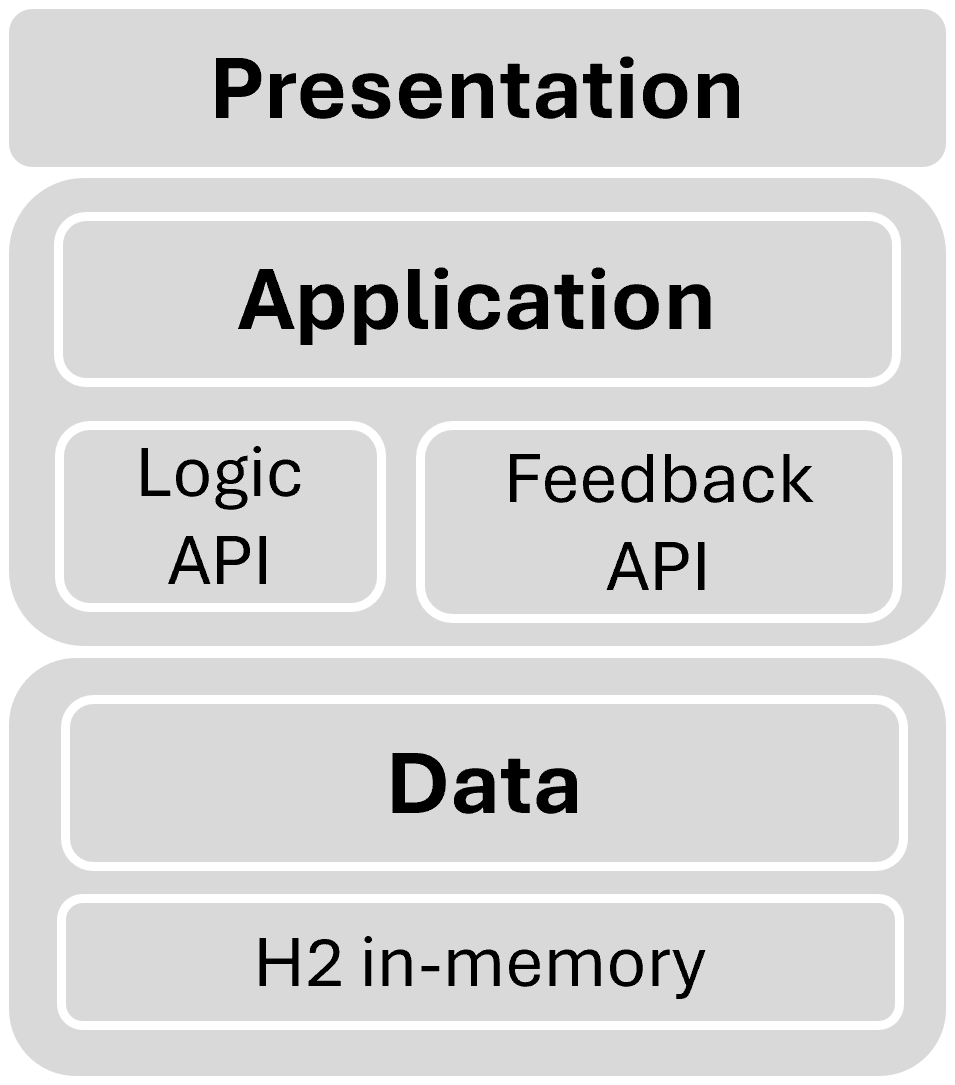
\includegraphics[width=0.35\linewidth]{Chapters/Figures/server-modules.png}
   \caption{Layers of the Application module}
    \label{fig:server-modules}
\end{figure}

Starting from the bottom, the Data layer is responsible for data storage, retrieval, and management. In this layer, we defined Data Transfer Objects (DTOs), which are used to safely exchange data between the backend and the website. We also implemented Data Access Objects (DAOs) for handling \gls{ND} problems, along with the corresponding Spring Data JPA repositories, which abstract interactions with the database and allow operations such as queries, inserts, and updates without writing SQL. Additionally, we provided initial content through predefined data inserts so that the problems table is populated with the exercises we want to display on the website. For the database, we use the H2 in-memory database [REF], which is lightweight and well-suited for the small amount of data currently stored, as we only handle exercises at this stage. Thanks to Spring’s abstraction, the system can be easily extended to support other relational databases or to store additional data objects without requiring significant changes to the existing codebase.

The next layer is the Application layer, which acts as an intermediary between the Data layer and the Presentation layer. This layer handles all core functionalities and data transformations, allowing changes in the system’s behavior without affecting the other layer. It contains the main methods that process \gls{ND} proof exercises, either by directly invoking functions in the Logic and Feedback APIs or by accessing data from the database. Within this layer, the proof object is further transformed into its final representation, which is the form sent to the website and used to generate the proof. \autoref{fig:nd-representations} clearly illustrates the different representations that a proof can have across the modules required for its proper validation.



\begin{figure}
    \centering
    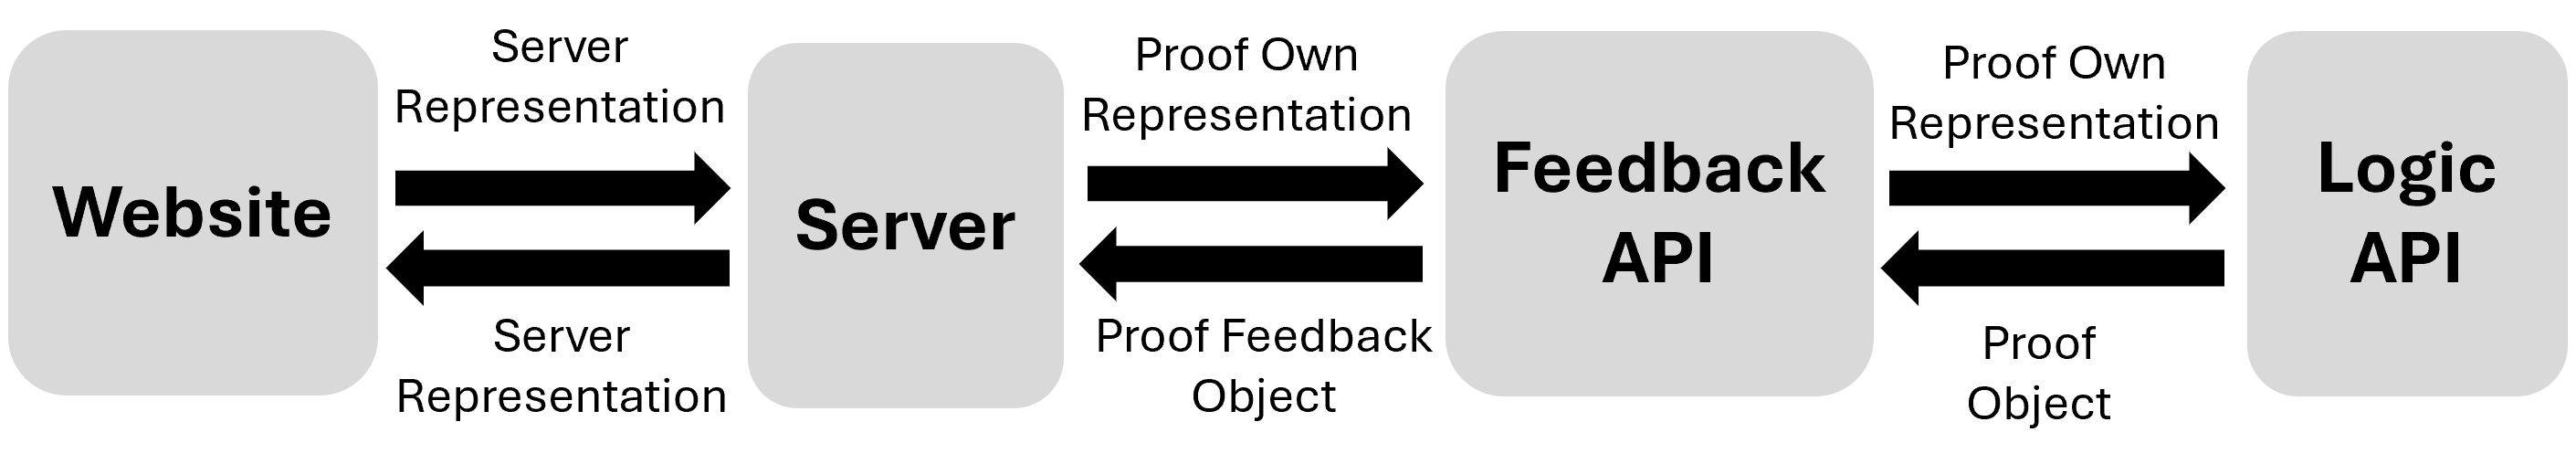
\includegraphics[width=0.95\linewidth]{Chapters/Figures/nd-representations.png}
    \caption{Different representations of a proof across the layers required for its validation}
    \label{fig:nd-representations}
\end{figure}

As we can see, the proof has different representations across the modules. Let us start from the website module. Suppose a student submits a proof for validation: the proof is first sent to the server in the server format, then converted into our own \gls{ND} proof language. This representation is maintained until it reaches the Logic module, where the proof is validated. On the way back, the responses from both APIs are Java objects representing the proof tree along with its associated data. Once the response reaches the server, the object is converted back into the server representation to simplify data handling in the website module.

\autoref{lst:sever-json} shows the JSON server representation for the same proof presented in \autoref{fig:nd-asts}. This representation differs from the feedback representation in several ways. It now tracks the types of the components (TREE, EXP, MARK, and RULE), which are used to build the proof tree on the website. Errors are represented as lists, allowing multiple errors to be attached to the same formula or rule if needed. Each field can also indicate whether it can generate hints, enabling users to request guidance for that part of the proof. Finally, the header of the object contains information about the conclusion, the premises, and the hypotheses of the current submission.

\begin{figure}[H]
\centering
\begin{minipage}{0.48\textwidth}
\begin{lstlisting}[language=json,
numbers=left]
{
  "conclusion": "(a ∨ a) → a",
  "premises": [
    "a ∨ a"
  ],
  "hypotheses": {
    "2": "a",
    "3": "a"
  },
  "proof": {
    "type": "TREE",
    "errors": {},
    "conclusion": {
      "type": "EXP",
      "errors": {
        "This tree doesn't solve the problem!\nYou proved:\n{a ∨ a} ⊢ (a ∨ a) → a"
      },
      "value": "(a ∨ a) → a",
\end{lstlisting}
\end{minipage}%
\hfill
\begin{minipage}{0.48\textwidth}
\begin{lstlisting}[language=json,
numbers=left,
firstnumber=last]
      "mark": null,
      "genHints": false,
      "env": {}
    },
    "marks": [
      {
        "type": "MARK",
        "errors": {},
        "value": "1"
      }
    ],
    "rule": {
      "type": "RULE",
      "errors": {},
      "value": "→I"
    },
    ...
  }
}
\end{lstlisting}
\end{minipage}
\caption{Example of the server JSON representation of a proof}
\label{lst:sever-json}
\end{figure}

The final layer is the Presentation layer, which provides the endpoints for communication with the client. In this layer, we define the API interface, specifying the operations that the client can perform. Before sending a response to the client, all messages are wrapped in an object that includes information about the HTTP status and the corresponding response code.

Now we list all operations available on our server API. The operations are divided into two groups: expressions and \gls{ND} proofs.

\begin{itemize}[label={}]
\setlength{\itemsep}{5pt}
    \item \textbf{Expressions:}\\
    These endpoints are used to check individual formulas within proofs. They improve responsiveness on the website by allowing verification of only the inserted formula instead of the full proof.
    \begin{itemize}[noitemsep, topsep=0pt]
    \setlength{\itemsep}{5pt}
        \item \textbf{POST /exp/pl}: Verifies a \gls{PL} formula provided in the request body and generates feedback according to the specified feedback level.
        \item \textbf{POST /exp/fol}: Verifies a \gls{FOL} formula provided in the request body and generates feedback according to the specified feedback level.
    \end{itemize}

    \item \textbf{Proofs:}\\
    These endpoints are related to \gls{ND} proofs. Similar to expressions, they are divided into \gls{PL} and \gls{FOL} categories.
    \begin{itemize}[noitemsep, topsep=0pt]
\setlength{\itemsep}{5pt}
        \item \textbf{GET /nd/pl/problem/\{problemNum\}}\\
        \textbf{GET /nd/fol/problem/\{problemNum\}}: Retrieves a specific \gls{ND} problem identified by the problem number in the URL path.

        \item \textbf{GET /nd/pl/problem}\\
        \textbf{GET /nd/fol/problem}: Retrieves a list of \gls{ND} problems, optionally paginated using the page number and page size query parameters.

        \item \textbf{POST /nd/pl}\\
        \textbf{POST /nd/fol}: Verifies a proof sent in the request body and provides feedback according to the specified feedback level.

        \item \textbf{POST /nd/pl/problem}\\
        \textbf{POST /nd/fol/problem}: Verifies whether a proof solves a problem, providing feedback according to the specified feedback level.

        \item \textbf{GET /nd/pl/problem/solve}\\
        \textbf{GET /nd/fol/problem/solve}: Solves a \gls{ND} problem using our algorithm, specified via the problem query parameter, and returns the solution.

        \item \textbf{POST /nd/pl/hint}\\
        \textbf{POST /nd/fol/hint}: Generates a hint for a \gls{ND} problem using the problem premises, goal conclusion, and feedback level.

        \item \textbf{GET /nd/pl/exps}\\
        \textbf{GET /nd/fol/exps}: Lists all possible formulas that can be obtained by decomposition for a given set of expressions. This is useful for the auxiliary keyboard, where it suggests which formulas can be introduced.

    \end{itemize}
\end{itemize}

In this module of the architecture, no security system has been implemented yet. In future work, we plan to extend this module to support user sessions. This would allow users to create mechanisms to save their solutions, track completed exercises, and monitor their proficiency levels. With this information, the system could automatically assign the appropriate feedback level, instead of relying on manual selection as it currently does. The application layout is designed to be easily extended, so integrating these features in the future should be straightforward.

\subsubsection{Tests}
Testing in this module was performed using mocking. We used MockMvc [REF], a testing tool provided by Spring that allows developers to simulate HTTP requests to controllers without starting a full web server. MockMvc is commonly used for unit and integration testing of Spring MVC applications, enabling verification of request handling, response content, status codes, and headers in a fast and controlled environment. 

One of the tests evaluated multiple modules of the application simultaneously. The test consisted of loading the full list of exercises for a given logic language using the appropriate endpoint. For each problem, we then queried its solution using the endpoint that computes solutions for \gls{ND} problems. Finally, for each solution, we verified whether the proof was correct using the endpoint that checks if a proof solves a problem. Additional tests were conducted to verify the functionality of the remaining endpoints.

\subsection{Website Service}
The last module of our application is the Website module, which is where users interact with the system through a web page. A full description of the graphical interface of the site can be found in [REF PROTOTYPE].

In this module, we use TypeScript [REF] as the main programming language and the React [REF] library to create an interactive system, which is one of the key features of our project. React is component-based, meaning applications are built from reusable components. Each component is responsible for rendering a small part of the UI and can detect changes to its state, automatically updating that part of the page. This allows React to efficiently update the DOM whenever the state changes.

Our first step in developing this module was to search for libraries that could provide a drag-and-drop environment for proofs. We found React Flow [REF], a powerful library for creating interactive node-based UIs that allow building graphs and pipelines. It seemed promising, but unfortunately the free version did not allow full manipulation of the drag-and-drop system. Since this library limited us to representing connections between proof elements through graph-like edges, while our planned approach relied on nesting and unnesting blocks, we decided to abandon it. Another library we found was the dnd-kit library [REF], a lightweight drag-and-drop library that supports the basic events needed to replicate nesting and unnesting actions. It was from this library that we started developing the webpage. Since it did not provide features for building an interactive node-based editor, we searched for another library to complement dnd-kit with screen navigation, zooming, and a minimap view. We found react-zoom-pan-pinch [REF], which provided exactly these features.

With all the necessary libraries in place, we were ready to implement the website module. We began by defining the pages our website would have and decided on two main pages: the first, where the user can select an exercise from a list of all available exercises, and the second, which provides the environment for building proofs. Since React is a component-based library, we had to define a separate component for each element on these pages.

\subsubsection{Components}
We will focus only on the proof-related components, although the logic for the remaining components is very similar. We started by identifying the components that make up a tree-shaped proof and ended up with five main components. The Tree component is the most important, as it provides the structure for the proof and can take two different forms: a simpler version for proofs with only one formula, and a composite version that can support rule applications. The Rule Names component specifies which rule is being applied and can be assigned to the tree. The Expressions component represents the formulas in the proof. Marks component can be assigned to both expressions and trees components. Finally, the Feedback Tooltips component can be attached to expressions or trees to display errors or hints to the users. \autoref{fig:web-components} shows an illustration of the different components that make up a proof representation.
 
\begin{figure}[h!]
    \centering
    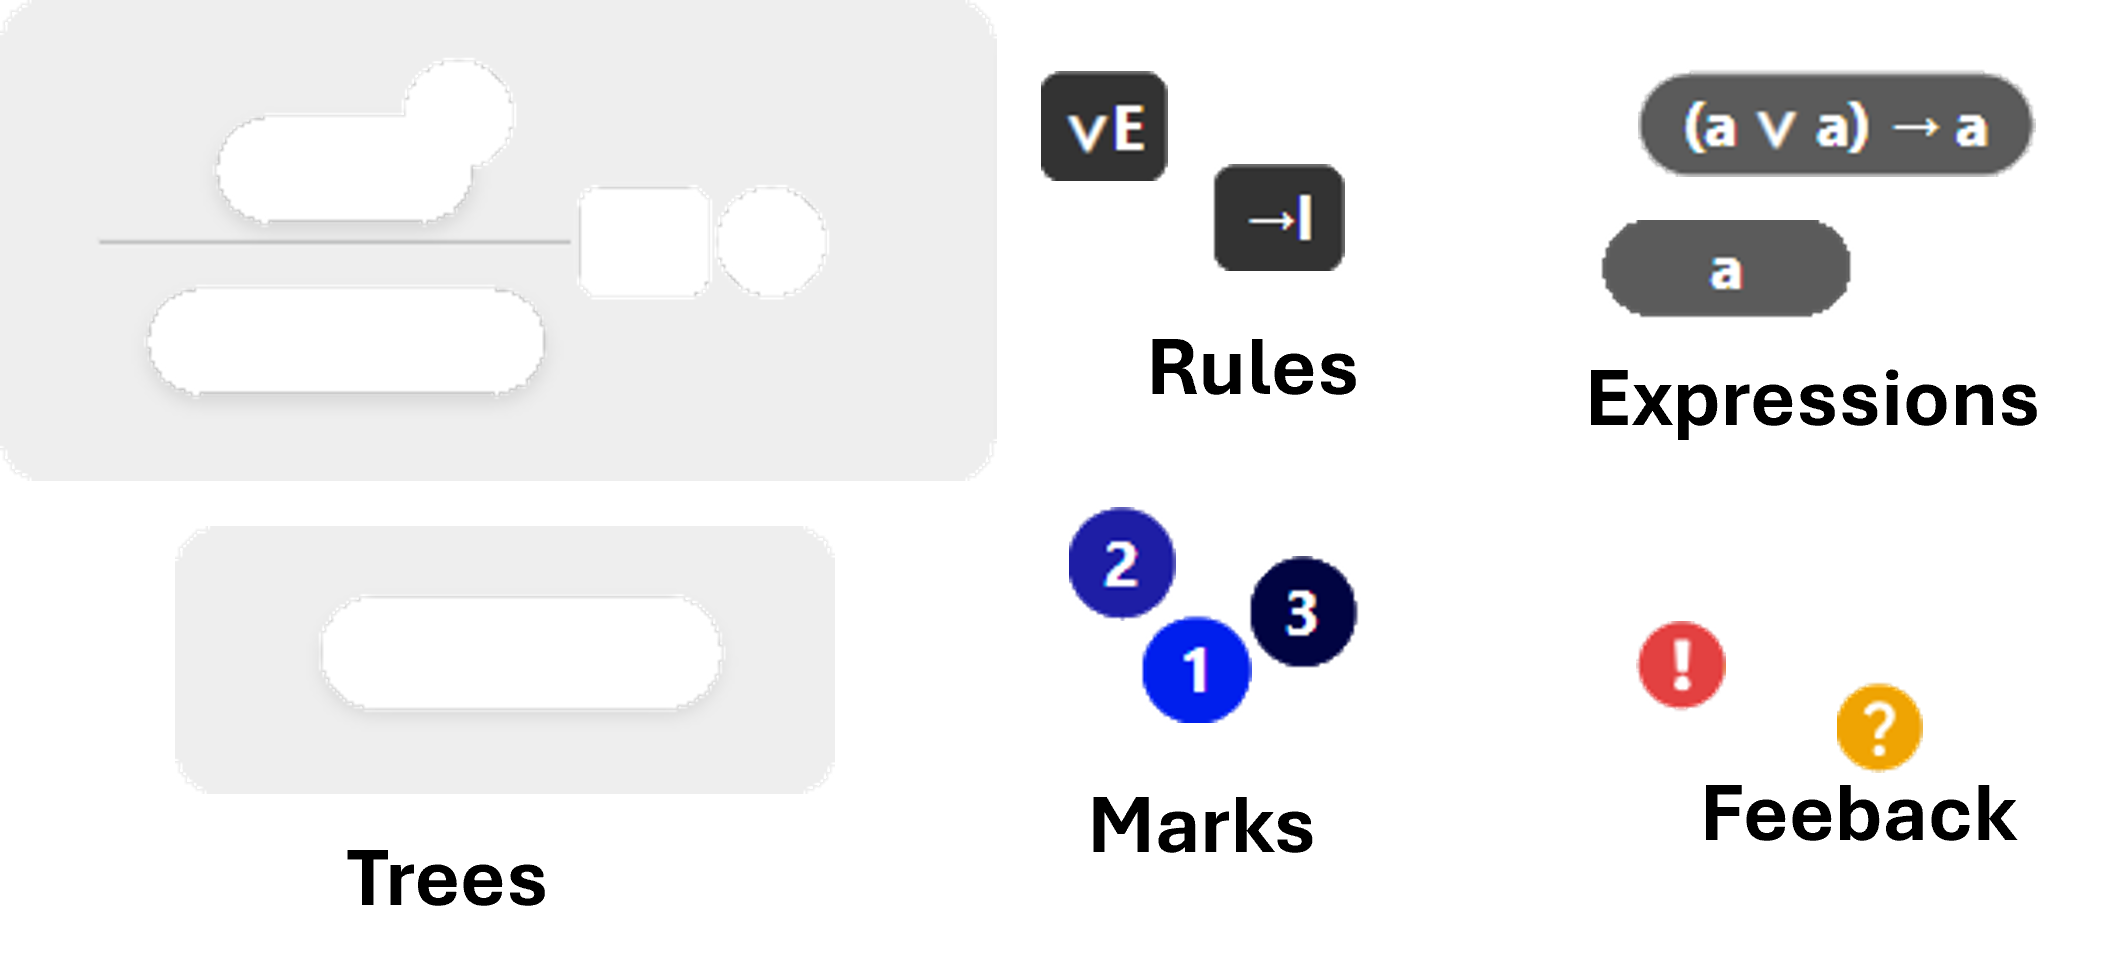
\includegraphics[width=0.90\linewidth]{Chapters/Figures/components.png}
    \caption{Different components that make up a complete proof representation in the system}

    \label{fig:web-components}
\end{figure}

Each component has its own hook, which extracts the logic of the component into a reusable unit. For the tree component we define the drag-and-drop events, specifying which elements can be dropped and which cannot. For the rule names and marks we implement the logic to trigger the corresponding selector component (the list of rules or marks). For the expressions we add the logic to activate the edit mode, which opens the auxiliary keyboard for inserting formulas, together with the logic for applying rules, assigning marks, and dragging the proof linked to that expression. Finally, for the feedback tooltips we include the logic to display textual errors or hints when the user hovers over or clicks on the component.

\subsubsection{REST API and Swagger}
Another important part of this module is the communication with the server. As explained in previous sections, the website and server modules interact through REST requests, where essential data is exchanged. To handle these requests we used Swagger [REF], a framework for describing and documenting REST APIs in the server module. Swagger includes a feature called Swagger Codegen, which can automatically generate client code or server stubs from an API description. This saved us a significant amount of time, since we only needed to run commands to generate the code to call operations from the server instead of writing it manually. It is also very valuable for future expansion, as we can easily add new endpoints to the server with different functionalities and automatically generate the corresponding TypeScript requests.

\subsubsection{Storage}
Focusing on data storage, we defined a class called Board to manage and maintain the state of the proof environment. This class stores information such as the exercise being solved, the learner's feedback level, the element currently being dragged, dropped, or edited, the components rendered on the board, the zoom level, and a stack of changes for undo and redo operations, among other details. To handle this complex state and ensure consistency across the interface, we integrated Redux [REF], a state management library for JavaScript and TypeScript applications. Redux centralizes application-wide state in a single store instead of distributing it across multiple components, which allows different parts of the application to share and update data in a reliable way. With Redux, the Board object’s state is synchronized across the entire interface, enabling features such as live updates without the risk of inconsistent or duplicated data.

Proof components, shown in \autoref{fig:web-components}, are identified by numbers stored in a map inside the Redux store. This choice was made to improve both efficiency and interactivity on the page. The numbers act as unique identifiers for the component objects stored in the store. For example, when a click event occurs on an expression, we can quickly use its identifier to retrieve the corresponding object from the store and access its value.

Why should we use an identifier? Imagine a proof environment with thousands of components rendered. If we had to traverse the entire list of components every time we needed information about a specific one, the process would be extremely time-consuming and would significantly harm the efficiency of the page. By using IDs as keys in a map, we can directly access the corresponding object, since accessing objects by their ID in a map is much faster than traversing a list.

Another feature that takes advantage of this approach is the ability to manipulate the data in the trees. Since all components are identified by numbers, we can use these references to define the tree interface, as shown in \autoref{fig:tree-interface}.

With this methodology, we can easily swap and move elements within proofs. For example, by simply replacing a number in the hypotheses array, we can simulate the drop event of a formula or a tree, depending on the type of object assigned to the new ID. We can also easily reorder elements within the hypotheses, move objects to different subtrees, and perform various other manipulations.

\begin{figure}
    \centering
    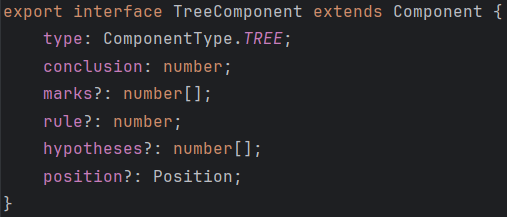
\includegraphics[width=0.70\linewidth]{Chapters/Figures/tree-interface.png}
    \caption{Interface for the tree component using references for the different elements that make up a tree component}
    \label{fig:tree-interface}
\end{figure}

During the rendering process, we start with a list of root elements stored in the Board object. For each root element, we recursively traverse its sub-elements, replacing references with the actual objects. This process continues until all references have been resolved and rendered on the interface.

But how do we convert the representation sent by the server (see \autoref{lst:sever-json}) into the indexed format used in the Board? In our Board, we maintain a field that tracks the last ID assigned to each component. Every time a new element is added, this field is incremented. We take the tree object returned from the server and assign a unique ID to each node. To display the full tree in the proof environment, we add the ID of the root node to the array of root elements stored in the Board. This array contains only the elements that can be placed directly on the proof environment.

This is how the proof environment processes components. This structure allows us to easily add new components, perform modifications efficiently, and render thousands of elements without lag, which is particularly important for less powerful devices.

\subsubsection{Sever communication}
Now let us describe the interactions between the website and the server. The first Interaction begins when the user enters the main page. The webpage sends a request to the server to load the list of exercises for both \gls{PL} and \gls{FOL}. When a user selects a problem, they are redirected to the proof environment, while in the background a request is sent to compute the auxiliary expressions (the ones shown on the auxiliary keyboard), and the response is stored in the Redux store. During proof construction, every time the user exits edit mode on a formula, the inserted formula is checked on the server, avoiding the need to submit the entire proof just to verify a single change. When a user submits a proof, a request is sent to the server to validate it, checking both whether the proof is correct and whether it solves the current problem. Clicking the hint button (the yellow one with the question mark icon) triggers a server request to generate a hint. This approach avoids pre-computing all hints every time a proof is submitted, improving performance.

This module provides a robust interface for users to practice \gls{ND} exercises. It was implemented with future expansion in mind, allowing additional pages for different exercises to be added without interfering with the existing implementation. Similarly, components can be easily reused or extended, making the system flexible and maintainable. The integration with Redux ensures that the state of complex interactions, such as proof construction and drag-and-drop operations, remains consistent and responsive. Overall, this module combines usability, efficiency, and scalability, forming a solid foundation for further development and improvements.

\subsubsection{Tests}
The website module was evaluated through user testing sessions (see [REF]) to ensure that the system is easy to use, quick to learn, interactive, and intuitive. These tests focused on assessing the overall usability and user experience of the interface.
